\documentclass[../main.tex]{subfiles}
\usetikzlibrary{calc,trees,positioning,arrows,fit,shapes,calc}

\begin{document}

\begin{definition}
    $f$ is called \textbf{one-to-one} if $f(x_1) \neq f(x_2)$ whenever $x_1 \neq x_2$ or equivalently
    \[
        f(x_1) = f(x_2) \implies x_1 = x_2
    \]
\end{definition}

\begin{figure}[H]
 \centering
 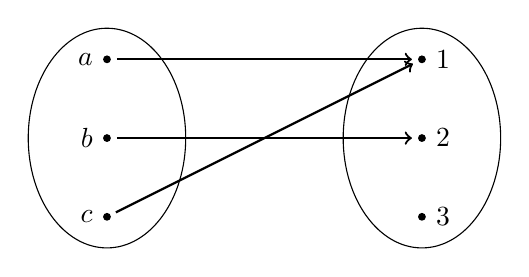
\begin{tikzpicture}[ele/.style={fill=black,circle,minimum width=.8pt,inner sep=1pt},every fit/.style={ellipse,draw,inner sep=-2pt}]
  \node[ele,label=left:$a$] (a1) at (0,4) {};
  \node[ele,label=left:$b$] (a2) at (0,3) {};
  \node[ele,label=left:$c$] (a3) at (0,2) {};

  \node[ele,,label=right:$1$] (b1) at (4,4) {};
  \node[ele,,label=right:$2$] (b2) at (4,3) {};
  \node[ele,,label=right:$3$] (b3) at (4,2) {};

  \node[draw,fit= (a1) (a2) (a3),minimum width=2cm] {} ;
  \node[draw,fit= (b1) (b2) (b3),minimum width=2cm] {} ;
  \draw[->,thick,shorten <=2pt,shorten >=2pt] (a1) -- (b1);
  \draw[->,thick,shorten <=2pt,shorten >=2] (a2) -- (b2);
  \draw[->,thick,shorten <=2pt,shorten >=2] (a3) -- (b1);
 \end{tikzpicture}
 \caption{A function which is not 1-1.}
 % http://tex.stackexchange.com/questions/19987/drawing-a-bijective-map-with-tikz
\end{figure}

\textbf{Horizontal Line Test.}
Let $f: \mathbb{R} \to \mathbb{R}$. By definition of a function any vertical line intersects the graph at one point. $f$ is 1-1 if its graph is never intersected by any horizontal line more than once.

\textbf{Increasing or Decreasing Functions are 1-1.}

\begin{definition}
    If $f$ is one-to-one then it has an inverse function $f^{-1}$ defined as follows: If $x$ is in the range of $f$ then it is in the domain of $f^{-1}$ and
    \[
        f^{-1}(x) = y \iff x = f(y).
    \]
\end{definition}

\begin{example}
    $f(x) = x^2$ is not 1-1 and so does not have an inverse.
\end{example}

\begin{example}
    Show that $f(x) = 2x -1$ is one-to-one and find its inverse $f^{-1}(x)$.
\end{example}
\begin{solution}
    Since $f'(x) = 2 >0$, $f$ is increasing on $\mathbb{R}$ and therefore one-to-one for all $x$. Let $y = f^{-1}(x)$, solve for $y$ to get
    \[
        f^{-1}(x) = \frac{x+1}{2}.
    \]
\end{solution}


\subsection*{Properties of inverse functions}
\begin{enumerate}
    \item The domain of $f^{-1}$ is the range of $f$.
    \item The range of $f^{-1}$ is the domain of $f$.
    \item $f(f^{-1}(x)) = x$ for all $x$ in the domain of $f^{-1}$.
    \begin{proof}
        If $f^{-1}(x) = y$ then $x = f(y)$ and
        \[
            f(f^{-1}(x)) = f(y) = x
        \]
    \end{proof}
    \item $f^{-1}(f(x)) = x$ for all $x$ in the domain of $f$.
    \item $(f^{-1})^{-1}(x) = f(x)$ for all $x$ in the domain of $f$. (The inverse of inverse of $f$ is $f$.)
    \begin{proof}
        \[
            (f^{-1})^{-1}(x) = y \iff f^{-1}(y) = x \iff y = f(x).
        \]
    \end{proof}
    \item The graph of $f^{-1}$ is the reflection of the graph of $f$ in the line $x=y$. (Because if $(a, b)$ is a point on the graph of $y=f(x)$ then $(b, a)$ is a point on the graph of $y = f^{-1}(x)$).
\end{enumerate}
\begin{figure}[H]
    \centering
    \includegraphics[scale=.5]{3-1-inversefunc}
    \caption{The graph of the inverse function is a reflection along $y=x$.}
\end{figure}

\subsection*{Inverting Non One-to-one Functions}
The function $f(x) = x^2$ is not one-to-one and hence not invertible. $f(-a) = f(a)$ for any $a$. Let us define a new function by restricting the domain of $f$
\[
    F(x) = x^2, \quad x \geq 0
\]
Then $F^{-1}(x) = \sqrt{x}$.
\begin{figure}[htbp]
    \centering
    \includegraphics[scale=.5]{3-1-inversex2}
    \caption{The restriction of $x^2$ to $[0, \infty)$ and its inverse.}
\end{figure}

\subsection*{Derivatives of Inverse Functions}
Let $y = f^{-1}(x)$.
\[
    \frac{d}{dx} f(y) = \frac{d}{dx} x \implies f'(y) \frac{dy}{dx} = 1 \implies \frac{dy}{dx} = \frac{1}{f'(y)}
\]
Thus
\[
    (f^{-1})'(x) = \frac{1}{f'(f^{-1}(x))}
\]

\begin{example}
    Show that $f(x) = x^3 + x$ is one-to-one on the whole real line and find $(f^{-1})'(10)$. Hint: $2^3 + 2 = 10$.
\end{example}
\begin{solution}
    First $f'(x) = 3x^2 + 1 >0$. Hence $f$ is 1-1.
    Let $y = f^{-1}(x)$.
    \[
        (f^{-1})'(x) = \frac{1}{3 y^2 + 1} = \frac{1}{3 (f^{-1}(x))^2 + 1}.
    \]
    \[
        (f^{-1})'(10) = \frac{1}{3 (f^{-1}(10))^2 + 1}.
    \]
    \[
        y = f^{-1}(10) \implies f(y) = 10 \implies y = 2 \implies f^{-1}(10) = 2.
    \]
    Thus
    \[
        (f^{-1})'(10) = \frac{1}{3\times2^2 + 1} = \frac{1}{13}.
    \]
\end{solution}

\begin{example}[OPTIONAL]
    Show that
    \[
        f(x) =
        \begin{cases}
            x^2+1, &\text{ if } x \geq 0\\
            x+1, &\text{ if } x < 0
        \end{cases}
    \]
    is 1-1 and find its inverse.
\end{example}
\begin{solution}
    $f'(x) > 0$ for $x<0$ and $x>0$ so it is increasing for $x<0$ and $x<0$. Also if $x<0$ then $f(x) < 1 = f(0)$ and if $x>0$ then $1 = f(0) < f(x)$, hence $f$ is increasing everywhere. That proves that $f$ is 1-1.
    \[
        f^{-1}(x) =
        \begin{cases}
            \sqrt{x-1}, &\text{ if } x \geq 0\\
            x-1, &\text{ if } x < 0
        \end{cases}
    \]
\end{solution}

\end{document}